% Kurzbez.  : Introduction - to draw a picture of the problem
%% Pagecount: 10
%%
%%

\section {Introduction}

The Open Linking and Embedding for Process Control (OPC) consortium
released several open standards, which address interfaces for vertical
integration in industrial automation. These standards can be used to
build Internet/fieldbus interfaces which are placed on gateway devices
as shown in figure \ref{inet_fb_gw}

\begin{figure}[ht]
\htmlborder{1}
\centering
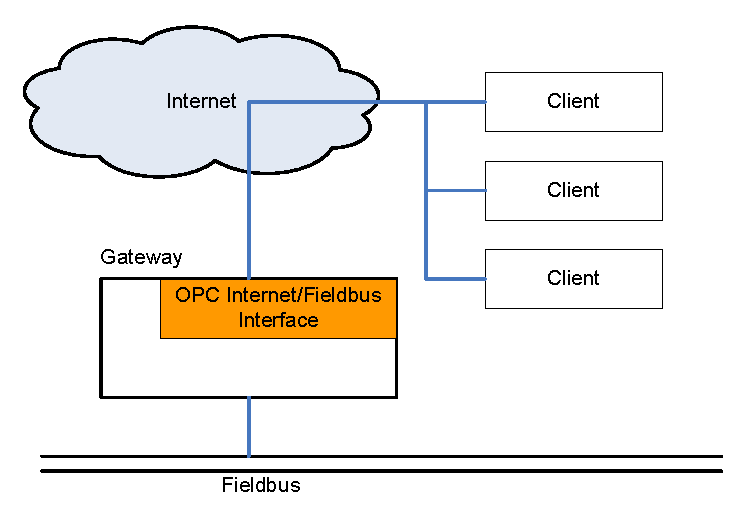
\includegraphics[scale=0.7]{graphics/inet_fb_gw.eps}
\caption{Internet/fieldbus interface on a gateway}
\label {inet_fb_gw} 
\end{figure} 

Historically, OPC used the Distributed Component Object Model (DCOM)
for the underlying communication technology. DCOM has the disadvantage
of being platform specific: it is only available for Microsoft
Windows based systems. Other platforms, such as Linux, can therefore
not retrieve fieldbus data from DCOM based servers. Another
disadvantage of DCOM is that it can not easily bypass firewalls, hence
access will often be limited to certain segments of a corporate
network.

In the last years, a new technology, called SOAP Web services, emerged.
\cite{SOAP2} defines a Web Service as: ``a method or function that is
available for other applications to access over the Internet.''. Web
services enable Remote Procedure Calls (RPC) and have the following
key features:

\begin{description}
\item[High level of interoperability:] Web services technologies are
all based on strictly defined open standards\footnote{Most
technologies are W3C standards.}.
\item[High networking abilities:] As an underlying communication
protocol, Web services utilize Internet protocols such as the Hyper
Text Transfer Protocol (HTTP) or the Simple Mail Transfer Protocol
(SMTP). These protocols have high networking abilities and may
moreover penetrate firewalls.
\item[Protocol legible by humans:] The Simple Object Access Protocol
(SOAP)\footnote{To be correct, SOAP is not an acronym for Simple
Object Access Protocol anymore, instead it's simply ``SOAP''.} is based
on the Extended Markup Language (XML), which is legible to
humans. This way, testing and debugging of Web services is far easier
than with binary protocols.
\item[Documentation:] Another underlying technology of SOAP is the
``Web Service Definition Language'' (WSDL) which may be used to define
the service, especially by constraining the format of the SOAP
protocol. WSDL utilizes the XML Schema language for defining these
SOAP messages\footnote{More information about XML Schema can be found
in \cite{XSD1}.}. These WSDL documents can be utilized by frameworks
to generate stubs that provide a base for accessing a Web service.
\item[Validation:] WSDL in combination with a validating XML parser
enable the validation of SOAP messages. This way, custom code will
never receive syntactically or semantically erroneous data, which
should improve the stability of the service.
\end{description}

SOAP Web services are seen as a successor to several alternative
technologies such as DCOM and are already broadly accepted by the
industry. More information about the SOAP protocol can be found in
\cite{SOAP1} and \cite{SOAP2}.

The OPC consortium reacted on this technological evolution by adopting
SOAP Web services for their standards. One recent addition of OPC is
the "XML Data Access Version 1.0" (XML-DA 1.0) standard. This standard
deals with access of underlying fieldbus technologies and covers the
following aspects:

\begin{description}
\item[Information model:] The specification provides a simple
information model, based on ``OPC Items'' which represent a piece of
information, similar to fieldbus data points. These items can be
arranged hierarchically.
\item[Data types:] OPC XML-DA adopts several XML-Schema based data
types, such as integer, float, date/time specific types. Moreover it
defines arrays which are based on these basic types.
\item[Operations:] The standard specifies 8 operations such as
reading/writing and browsing which can be used to access the
underlying fieldbus.
\item[Subscription:] The specification further introduces a mechanism
to retrieve only changed items, called ``Subscription''.  Clients may
thus subscribe to items and use a dedicated polling operation to
retrieve changed data.
\end{description}

The standard does not address security, instead it relies on
underlying Web service technologies\footnote{For instance, HTTPS can
be used to secure a HTTP channel.}. More information about OPC XML-DA
can be found in \cite{diplomarbeit} and \cite{OPCXMLDA}.

Although OPC XML-DA is based on open and standardized technologies, it
can nevertheless be tedious to build services based on this standard.
Therefore several OPC frameworks are available that introduce simple
building of client and server applications. However, most of these
frameworks are not freely available, moreover most of them are based
on Microsoft's .Net framework and are therefore platform dependent.

Due to these limitations, the PyOPC framework was developed, which
fully implements the OPC XML-DA standard, enabling developers to build
OPC XML-DA based applications in an easy way.
